%% ---------------------------------------------------------------------------
%%  REVIEW COPY / PRE-SUBMISSION DRAFT
%%
%%  Same text as paper.tex -- both pull body.tex and refs.tex -- but laid out
%%  for reading and annotation: single column, 1.5 spacing, numbered lines,
%%  wide right margin for comments.
%%
%%  Edit the manuscript text in body.tex, NOT here and not in paper.tex.
%%
%%  Compile with:  pdflatex paper-draft   (three times, for cross-references)
%% ---------------------------------------------------------------------------
\documentclass[11pt,oneside,a4paper]{article}

\usepackage[T1]{fontenc}
\usepackage[utf8]{inputenc}
\usepackage{amsmath,amssymb}
\usepackage{newtxtext,newtxmath}

%% Wide right margin: room to write comments next to the text.
\usepackage[a4paper,top=2.5cm,bottom=2.5cm,left=2.6cm,right=4.6cm,
            marginparwidth=3.4cm]{geometry}
\usepackage{graphicx}
\usepackage{booktabs}
\usepackage{multirow}
\usepackage{array}
\usepackage{caption}
\usepackage{fancyhdr}
\usepackage{cite}
\usepackage{algorithm}
\usepackage{algpseudocode}
\usepackage{url}
\usepackage{enumitem}
\usepackage{setspace}
\usepackage{xcolor}
\usepackage{etoolbox}

%% ---- line numbers for annotation -------------------------------------------
\usepackage{lineno}
%% lineno loses display equations unless the amsmath environments are patched.
\newcommand*\patchAmsMathEnvironmentForLineno[1]{%
  \expandafter\let\csname old#1\expandafter\endcsname\csname #1\endcsname
  \expandafter\let\csname oldend#1\expandafter\endcsname\csname end#1\endcsname
  \renewenvironment{#1}%
     {\linenomath\csname old#1\endcsname}%
     {\csname oldend#1\endcsname\endlinenomath}}
\newcommand*\patchBothAmsMathEnvironmentsForLineno[1]{%
  \patchAmsMathEnvironmentForLineno{#1}%
  \patchAmsMathEnvironmentForLineno{#1*}}
\AtBeginDocument{%
  \patchBothAmsMathEnvironmentsForLineno{equation}%
  \patchBothAmsMathEnvironmentsForLineno{align}%
  \patchBothAmsMathEnvironmentsForLineno{gather}%
  \patchBothAmsMathEnvironmentsForLineno{multline}%
}

%% ---- captions (same wording as the submission layout) ----------------------
\DeclareCaptionLabelFormat{jcstfig}{\textbf{#1#2}}
\DeclareCaptionLabelFormat{jcsttab}{#1~#2}
\captionsetup[figure]{labelformat=jcstfig,labelsep=period,font=small,
                      justification=raggedright,singlelinecheck=false}
\captionsetup[table]{labelformat=jcsttab,labelsep=period,font=small,
                     justification=centering,singlelinecheck=false}
\renewcommand{\figurename}{Fig.}
\renewcommand{\tablename}{Table}

%% ---- DRAFT marking ---------------------------------------------------------
\newcommand{\draftversion}{draft 1}
\pagestyle{fancy}
\fancyhf{}
\renewcommand{\headrulewidth}{0.4pt}
\fancyhead[L]{\footnotesize\bfseries DRAFT \normalfont\footnotesize
              --- not for circulation or submission}
\fancyhead[R]{\footnotesize\thepage}
\fancyfoot[L]{\footnotesize Parayil --- Speaker credit history leaks the target
              in LIAR --- \draftversion, \today}

%% ---- theorem-like environments ---------------------------------------------
\newtheorem{definition}{Definition}
\newtheorem{proposition}{Proposition}
\newtheorem{theorem}{Theorem}

%% ---- spacing ---------------------------------------------------------------
\onehalfspacing
\setlength{\parindent}{1.2em}
\setlist[itemize]{leftmargin=1.4em,itemsep=2pt,topsep=4pt,parsep=0pt}
\setlist[enumerate]{leftmargin=1.7em,itemsep=2pt,topsep=4pt,parsep=0pt}
\renewcommand{\arraystretch}{1.1}
\setlength{\tabcolsep}{5pt}
\raggedbottom
%% Runs of \texttt{} filenames and inline math cannot hyphenate; let TeX stretch
%% the interword glue on those lines rather than overrun the wider measure.
\setlength{\emergencystretch}{3em}

\newcommand{\bs}[1]{\boldsymbol{#1}}
\newcommand{\best}[1]{\textbf{#1}}

%% ---- figure widths, scaled for the single-column measure -------------------
\newcommand{\figfull}{0.62\textwidth}
\newcommand{\figmed}{0.58\textwidth}
\newcommand{\fignarrow}{0.42\textwidth}
\newcommand{\figwide}{0.88\textwidth}

%% Tables and floats are \footnotesize in the body; keep them single-spaced so
%% they stay compact next to 1.5-spaced running text.
\AtBeginEnvironment{table}{\singlespacing}
\AtBeginEnvironment{table*}{\singlespacing}
\AtBeginEnvironment{algorithm}{\singlespacing}
\AtBeginEnvironment{thebibliography}{\singlespacing}

\hyphenation{mis-in-for-ma-tion clas-si-fi-ca-tion PolitiFact}

\begin{document}
\linenumbers

%% ===========================================================================
%%  FRONT MATTER
%% ===========================================================================
\begin{center}
{\large\bfseries Speaker Credit History Leaks the Target in LIAR:\\[3pt]
 A Leakage-Free Benchmark for Fine-Grained Fake News Detection}\\[14pt]
{\normalsize Aaron Koshy Parayil\quad and\quad Krishna Presannakumar}\\[5pt]
{\small\itshape Department of Computer Science, Christ University,
 Yeshwanthpur Campus, Bengaluru 560073, India}\\[3pt]
{\small E-mail: aaron12parayil@gmail.com,
 krishna.presannakumar@christuniversity.in}\\[6pt]
{\footnotesize\bfseries \draftversion\ --- \today}
\end{center}


\vspace{10pt}
{\singlespacing\small
\noindent\textbf{Abstract.}
%% Abstract body only -- no heading, no size command. Included by paper.tex.
The LIAR benchmark includes five ``credit history'' columns per speaker, but the
publication describing the data set notes that these include the statement to be
predicted, thus emphasizing that these should only be used after the current
annotation has been subtracted from it. We provide the evidence for the cost of
following these instructions. Forests fed with only those five columns from the
data set achieve 0.394 accuracy at the test time in the six-way classification
task, but the amounts achieved in the experiment when highlighting the value of
those columns according to what was stated in the paper when subtracting the
current label are equal to 0.659 against the majority class accuracy of 0.208.
Our proof comes from the counting rather than reasoning related to the algorithm
as to how it works. There are 3\,318 speakers who share 392 distinct counting
vectors in total, meaning that the vector used for this subtraction can be
treated as a deviation from a landmark that can be remembered by the classifier
and that this vector indicates the actual label as it retrieves the same value
for 36.2\% of the test rows. Subtraction is insufficient for the independent
reasons since the counts in question may be correlated as they are aggregated
across training, validation and test samples for 2\,846 of the defined number of
speakers. We then reconstruct speaker history according to three principles as
far as the training labels, out-of-fold coding and prior smoothing are
concerned, thus demonstrating that the model returns 0.228 score according to
the history approach, which is better than the primary class score. Finally, we
test six classifiers in a set of experiments under a protocol that selects on
validation and scores on testing once; the best configurations in this case
return 0.285 for six-class and 0.673 for binary accuracy, and the hybrid
configuration has performed better than both single modalities in cases.


\vspace{6pt}
\noindent\textbf{Keywords:} credit history, data leakage, fake news detection,
LIAR dataset, text classification
}

\vspace{10pt}
\hrule
\vspace{6pt}

%% ---------------------------------------------------------------------------
%%  Shared manuscript text
%% ---------------------------------------------------------------------------
%% Body of the manuscript -- text by Aaron Koshy Parayil.
%% Tables live in ./tables and are generated from the experiment outputs.

\section{Introduction}

The speed of misinformation is greater than the speed of institutions established to eliminate this misinformation. One false statement is able to form a public opinion long before it can reach the verification stage. At the same time, the number of false statements produced every day in social networks, political speeches, and news aggregators is much bigger than what any group of fact-checkers can handle. The effect of misinformation being distributed faster than verified is what leads to the need for automation in this process.

The initial approaches proposed for solving the problem included classifying statements as either true or false. This approach is rather convenient but it does not represent the reality of how the political statements work. One can express the fact correctly but without mentioning the circumstances surrounding it. The organization that checks the facts realized that long ago and started rating statements on a scale from true to false --- true and mostly true, half true, barely true, false, and pants on fire.

The LIAR dataset \cite{wang2017liar} was put together with the purpose of having the more difficult version of the task at hand. The dataset consists of 12.836 brief statements from PolitiFact, their six possible verdicts, and certain metadata of the speaker: his or her party, state of residence, job position, the subject of the statement, the place of making the claim, and five integer columns showing how often that speaker was rated as some slightly true, false, half-true, mostly true, or lying. The five columns with the counts of the way the speaker was rated are characteristic for the dataset as they carry information about the relations and background necessary for prediction which cannot be obtained from a 20-word sentence, and practically any research that adds metadata while using LIAR dataset is based on the data obtained in the last five columns. The fact that the five columns contain the statement which is the subject of prediction is not new and we do not say so. Wang \cite{wang2017liar}, who created the dataset, says it in the paper introducing the dataset mentioning that we need to exclude the current statement from its credit history. The README file of the dataset repeats this information, but Wang also suggests the problem of data leak.

When the prescribed calculation is performed, the leak does not disappear; instead, it becomes larger. Specifically, on the dataset tested with only the five credit-history columns, using a random forest results in the accuracy of six-class prediction reaching only 0.394; however, when the forest is tested with these columns but with the outcome value calculated according to stated instructions subtracted, the accuracy jumps to 0.659. In other words, by using the dataset after the re-calculation suggested by its author, the outcome becomes almost three times greater than the majority class outcome equal to 0.208.

The reasons behind this are structural, and this paper contributes to understanding the mechanism. Because the vector for each speaker is unchanging across all of the speaker's rows, and 3\,318 speakers share only 392 different worn vectors, the vector that has had its label subtracted is the distance from the point which the model memorizes, and the direction of this distance is what the label is. Presence in the test sample indicates that the label for 36.2 of rows is defined directly by the subtracted vector.

The subtraction method itself has yet another disadvantage. It bases the whole procedure on self-inclusiveness. All the counts are summed across the training, validation, and testing datasets thus the training row uses a summary that counts all labels of other sentences pronounced by the same speaker. Both of these issues can be defined using the term "target leakage" introduced by Kaufman and co-authors \cite{kaufman2012leakage}, which means that the target information during the training is available but it does not exist during the prediction. Fixing the problem would result in a different conclusion. When constructing the speaker chronicles, it is necessary to work with the training labels only, calculate the out-of-the-fold states in a way that the particular utterance is not involved in the speech features and smooth the data to make the low-frequency speakers be unable to generate saturated features. Thus, the isolated model provides the result of 0.228 which is very close to 0.208 that is the maximum one when using the majority class label.

\subsection{Contributions}

This paper has the following contributions.

\begin{itemize}
\item The essential calculation of correction is given and not both in operation (in Section 3.4). As recommended in (Wang), the process of getting rid of the actual label increases the history-only six-class accuracy from 0.3944 to 0.6594 rather than decreasing it, as it was mentioned before. To the best of our knowledge, this effect has never been calculated before.
\item A way of understanding why this calculation is made instead of an argument (in Section 3.5). There are only 392 different counting vectors for all the 3318 speakers, which allows us to say about the invertibility of matrix B - e, which produces the label with an accuracy of 36.2\% and narrows the possible results to an average of 3.61 options for six classes. It is stated under which conditions the self-exclusion makes leakage even bigger rather than preventing it from happening.
\item Another different reason, making it impossible for subtraction to succeed (in Sections 3.2 and 3.6). Those counts are calculated for three settings, for all the 2846 speakers of 2947 alike.
\item Leakage-free encoder for speaker history relying on three key concepts: train-only label assisting, out-of-fold encoding, and smoothing proportions prior with auxiliary features assisting to ascertain the score based on the history data.
\item New benchmark using six classifiers assessed with three types of features (text, metadata, and hybrid) applied in two tasks. Assessment is performed according to the procedure of making all selections on validation split and assessment of the test split conducted just once.
\item Practical suggestions for LIAR's future work in respect of dealing with sent columns, creating proper baseline, which comparisons can be published, and which cannot.
\end{itemize}

It is critical to understand there is restriction on the discussions in this paper concerning only classical and completely reproducible models and ideas.

Therefore, the main problem solved in this paper is related not to the modeling, but to finding a measurement approach, which matters greatly.

\subsection{Organisation}

In Section 2 the related work on comparable paradigms that have been utilized for LIAR is examined, and how this paper fits within it. The dataset is described and leakage audit is presented in Section 3. Section 4 talks about the modified pipeline. The experimental setup is presented in Section 5, exploratory analysis in Section 6, and results in Section 7. Section 8 interprets the significance of corrected figures for the literature and mentions the study limitations. Section 9 concludes the paper.

\section{Related Work}

In its early days, most research in this field viewed fake news detection as a binary classification task. While this approach made the process of gathering information easier, it also reveals the potential shortcomings of determining the truthfulness of a statement, as any statement people make rarely falls within the boundaries of right or wrong but is rather determined by several other factors including the originator of the statement, context, and elements left out of the statement. Therefore, making the necessary evaluations of the statement is not an easy task, and this is the main point of the LIAR research.

\subsection{Feature-Based Models and Their Ceiling}

LIAR was devised to allow the area progress beyond binary categories, such as evaluation of around 12800 claims on six-point scale, taking into account the speaker metadata. The traditional methods produce around 0.27 accuracy on six categories. It actually implies more about complexity of the process that has to be performed in a case of non-binary categorization. The following method provided fact-checkers' reasoning along with the claim and applied two-way LSTM achieving 0.36 results. Although it is a great step forward, the text is produced after the judgment is made hence it hardly can be called a similar task as in a case of working with the claim meaning only. It is also important to mention because it should be compared to the work with credit history columns in the same category case: feature that encodes the appropriate result generates great figures but unusable models. In another case, CNN-LSTM performed on Hindi news provide satisfactory results in this language, although transfer possibility was not proved.

\subsection{Modelling Speakers as a Network}

One method that researchers employed was that of creating a graph that exists over the speakers, parties, and claims made. The process of claims detection has been approached as a node classification issue with the help of the GNN technique. The results of that approach were approximately 0.38 but how every time where the graph failed to show the speaker, there was a decrease in performance (which occurs quite often not only in this setting but even in their dataset with 15.6\% from all test statements related to speakers with the missing training). There has been a more recent method that combined transformer architecture and GNN architecture that achieved the result close to 0.46 but it was associated with additional costs. A co-attentional graph neural network used in getting the information from user models produced much more qualitative results, especially for GossipCop and PolitiFact datasets but their nature is different from that of LIAR and it will not be possible to evaluate them directly. Various teams started using attention-based encoder directly in their work with BERT fine-tuning leading to a result of 0.41 and the issue of 512 tokens is not a concern.

\subsection{Large Language Models and Efficient Fine-Tuning}

With the emergence of increasingly sophisticated models came a change in direction in respect of research inquiry as well as research priorities. While prior research was focused on the quality of representation, the attention was shifted to the costs associated with adaptation. Task-specific and prefix tuning of GPT-2 avoided full retraining \cite{zhou2023fine} but were affected by wording of prompts used. DeBERTa-v3 made use of higher computation resources to produce around 0.47 \cite{martinez2024deberta}. LLaMA-2 and Mistral were evaluated in the few-shot mode without Fine-Tuning \cite{kumar2024combating}. Five prompts produced around 0.46 results while incurring a higher inference overhead. The highest performance came from the combination of pre-trained large encoders with Fine-Tuning, that allowed for achieving around 0.48 accuracy (of six-way tasks) and approximately 0.90 accuracy of the prediction (for BERT, RoBERTa, and DeBERTa) \cite{alqadi2025transfer}, as well as similar performance boost from adoption of LoRA to Mistral-7B \cite{thompson2025parameter}, and also over 0.99 accuracy from light-weight adapters \cite{alghamdi2025abert}. Mixture-of-experts paradigm was used in LLaMA-3.1 to route prompts and data to experts, thus achieving around 0.49 \cite{garcia2026hybrid}.

\subsection{Generalisation, Explainability and Robustness}

Issues concerning the practicality of deep learning can be examined in addition to those regarding its accuracy. The performance of cross-dataset transfer has been found to be rather poor. However, domain adversarial training is reported to produce a moderate score in terms of F1 in cross-domain applications \cite{patel2025cross}. Explainability has been studied with the use of attribution methods via DeBERTa \cite{nguyen2025explaining}. Moreover, the problem of robustness against possible distortions is still open; to be precise, the application of adversarial training failed to demonstrate the desirable effect in counteracting distortions inflicted by the GPT-4o \cite{almansoori2025adversarial}.

\subsection{Leakage and Evaluation Hygiene}

The methodological sources on which this paper is based are quite dated and doesn't relate much to research on misinformation. Kaufman et al. \cite{kaufman2012leakage} give the most common definition of leakage as sharing information about the target that wasn't available during the prediction phase, and stress that leakage is usually detected due to astonishingly high performance, not due to code verification. Out-of-fold construction of target-based features and blending of per class statistics with the global prior is a common procedure for high-cardinality categorical encoding \cite{miccibarreca2001preprocessing}; the technique described in Section 4.3 utilizes this technique for the leakage found in publicly accessible files rather than being manually implemented by the modeler. In terms of evaluation, Gorman and Bedrick \cite{gorman2019standard} prove that the conclusions drawn from a regular split are not verified in resampling, while Dodge et al. \cite{dodge2019show} claim that reported test results are meaningless without knowing the size of the search the results are based on.

\subsection{Relation to Prior Work on These Columns}

The paper pertains to a problem with a widely used benchmark, thus it is important to distinguish between what is previously known from what is being established in the present work.

What is already known is that the credit history count includes the label being predicted, according to Wang \cite{wang2017liar} in his original paper about LIAR and also in the dataset README when he refers to ``the total credit history count including the current label''. Moreover, Wang gives an advice on how to correct it: one needs to subtract the current label.

That the metadata presented in LIAR is exaggerated has been noted before, which means that nothing stated here constitutes a novelty for someone who is familiar with the dataset paper, who, thus, would only be surprised by the first of our audit rows in Table~\ref{tab:audit}.

What is established in the present work is four things. First, the proposed correction does not help to eliminate the leakage but instead expands it to a value of 0.6594 regarding the history-only six-class accuracy. Secondly, the failure phenomenon is elucidated instead of being discussed, which is expressed numerically, 3.318 individuals were researched who came from only 392 distinct counting vectors, hence it is appropriate to calculate directly the gone-away vector or to get a label with a precision of 36.2\%. Thirdly, it can be regarded as inappropriate for another reason either as it collects values from training, validation, and testing stages, which makes it less perfect. Fourthly, it points to the existence of one structure where there is no problem of leakage of the values and with the help of corrected baseline grid: two types of tasks, three companies, and six models.

This discrepancy in understanding is important for the overall interpretation of the article. No matter how strange it sounds, the third section is not about the discovery, it rather delivers possibilities to quantify the impact of the defect and understand why the restoration cannot be successful.

\subsection{Positioning}

We investigate the notion that benchmark metadata can be used in a distributed manner but demonstrate that this is not true. In terms of impact, we do not provide an alternate accuracy test since there is no classical mechanism that can operate against a well-tuned encoder. We suggest the modified measuring algorithm, the new feature design, and the benchmark scores.

\section{The LIAR Corpus and a Leakage Audit of Its Credit History}

\subsection{Corpus and Fields}

LIAR \cite{wang2017liar} has released 12.836 short utterances sourced from PolitiFact, resulting in three headerless tab-separated files. Each of the rows has 14 fields: the statement ID, the verdict (which is in six-way) statement text, a list of subject tags that is separated by commas, the speaker's name, the position he/she holds, the state of origin, and the five integer figures of the credit history, and the environment in which the utterance was made, which is either a speech or a statement. The table below shows a sample of the utterances along with each of them.

\begin{table}[t]
\caption{Fields of the LIAR corpus, measured over all 12\,836 rows}
\label{tab:fields}
\centering
\footnotesize
\begin{tabular}{@{}llrr@{}}
\toprule
Field & Type & Distinct & Missing \\
\midrule
\texttt{id}            & identifier   & 12\,836 & 0.00\% \\
\texttt{label}         & ordinal, 6 levels & 6  & 0.00\% \\
\texttt{statement}     & free text    & 12\,810 & 0.00\% \\
\texttt{subject}       & multi-label tags & 144 tags & 0.00\% \\
\texttt{speaker}       & categorical  & 3\,318 & 0.00\% \\
\texttt{job\_title}    & categorical  & 1\,348 & 27.86\% \\
\texttt{state}         & categorical  & 70     & 21.46\% \\
\texttt{party}         & categorical  & 24     & 0.00\% \\
\texttt{context}       & categorical  & 5\,080 & 1.00\% \\
\texttt{*\_c} (five columns) & integer counts & 392 vectors & 0.00\% \\
\bottomrule
\end{tabular}
\end{table}


The six verdicts represent an ordinal scale starting from taking off pants (the untruth in terms of the messages) and going through false, barely true, half-true, and mostly true ending at true. The data used in this research contains 10.269 training statements, 1284 validation statements, and 1283 test statements. The author preserved the original division into training, validation, and test data as it was necessary for being able to compare the results that are obtained for this corpus with the results from other published studies. The table gives the total number of distributions for each data set.

\begin{table}[t]
\caption{Label distribution across the official LIAR splits}
\label{tab:splits}
\centering
\footnotesize
\begin{tabular}{@{}lrrrr@{}}
\toprule
Label & Train & Valid & Test & Corpus \\
\midrule
\emph{pants-fire}  &   842 & 116 &  92 & 1\,050 \;(8.18\%) \\
\emph{false}       & 1\,998 & 263 & 250 & 2\,511 \;(19.56\%) \\
\emph{barely-true} & 1\,657 & 237 & 214 & 2\,108 \;(16.42\%) \\
\emph{half-true}   & 2\,123 & 248 & 267 & 2\,638 \;(20.55\%) \\
\emph{mostly-true} & 1\,966 & 251 & 249 & 2\,466 \;(19.21\%) \\
\emph{true}        & 1\,683 & 169 & 211 & 2\,063 \;(16.07\%) \\
\midrule
Total              & 10\,269 & 1\,284 & 1\,283 & 12\,836 \\
Majority share     & 0.2067 & 0.2048 & 0.2081 & 0.2055 \\
True-leaning share & 0.5621 & 0.5202 & 0.5666 & 0.5584 \\
\bottomrule
\end{tabular}
\end{table}


Five classes out of the six form approximately the same percentage ranging from 16\% to 21\% of the entire corpus and only the first one taking off pants has reached 8.18\%. This is quite unlike other binary datasets on misinformation.

\begin{table}[t]
\caption{Structural audit of the shipped credit-history columns}
\label{tab:audit}
\centering
\footnotesize
\begin{tabular}{@{}lr@{}}
\toprule
Property & Measurement \\
\midrule
Count vector is constant per speaker & 3\,314 / 3\,318 \\
Counts equal the speaker's tally over & \multirow{2}{*}{2\,846 / 2\,947} \\
\quad train $\cup$ valid $\cup$ test & \\
Single-statement speakers whose counts & \multirow{2}{*}{1\,689 / 1\,701} \\
\quad one-hot encode their own label & \\
\emph{true}-labelled single-statement speakers & \multirow{2}{*}{355 / 355} \\
\quad with an all-zero count vector & \\
Distinct count vectors across the corpus & 392 \\
\bottomrule
\end{tabular}
\end{table}


\subsection{Two Worked Examples}

One can understand the abstractions easily by looking at two specific rows from the corpus.

\textbf{Self-inclusion.} Since the first row of train.tsv refers to the speaker dwayne-bohac, who is associated with the false label and has a vector like (0, 1, 0, 0, 0) in the column of (barely\_true, false, half\_true, mostly\_true, pants\_fire) one can say that he has only one statement recorded in the corpus. The row contains a single value in the vector which refers to that particular statement. When a model probes into the second unit in the first row it simply reads its label and no amount of regularization on the model will improve the situation, although this property has been indicated by Wang in one of his publications as a property users should correct for.

\textbf{Cross-split aggregation.} The speaker John Edwards makes a total of 15 statements consisting of 12 training statements, 2 validation statements, and 1 test statement. All of these 15 rows contain the same vector (0, 2, 4, 4, 1) which is the sum of the claims made by that speaker in the entire corpus. The training rows alone would give (0, 1, 4, 4, 0). The only difference here is that the 2 validation statements, one true and the other false, are used in this case to generate the aggregate features seen in the 12 training rows. The test statement labeled true does not provide any additional information because the true\_c bucket is absent; had this statement been labeled otherwise, training would have made use of this true label in exactly the same way.

Both of these examples do not involve any peculiar speaker. The first row is the very first row of the file, and the second speaker is just an ordinary politician making an ordinary number of claims.

\subsection{Effect Size}

The structure itself doesn't provide information on the leak's precision, so we measure it. A random forest (with 100 trees, max depth of 25, seed number 42) is trained on just the five counting columns, with no statement texts, political party information, or state data available. The results for the six-class task can be found in Table~\ref{tab:effect} and in Fig.~\ref{fig:leakage}, which show that just five columns of integers (with no knowledge of what was said) yield a score of 0.3944, which is nearly two times higher than the majoritarian base rate and significantly better than the initial 0.274 reported for a hybrid model with convolutional architecture that included statement text \cite{wang2017liar}. The difference between the two values is a signature shown by Kaufman et al. \cite{kaufman2012leakage}: the result is too good given the input information.

\begin{table}[t]
\caption{History-only random forest on the six-class task, under four
constructions of the same underlying signal}
\label{tab:effect}
\centering
\footnotesize
\begin{tabular}{@{}lcc@{}}
\toprule
Construction & Test acc. & Macro-F1 \\
\midrule
Raw LIAR counts (as shipped)   & 0.3944 & 0.4056 \\
Prescribed fix $\bs{b}-\bs{e}_y$\rlap{$^\ast$} & 0.6594 & 0.6633 \\
Leak-free out-of-fold history  & 0.2284 & 0.2236 \\
\midrule
Majority class                 & 0.2081 & --- \\
\bottomrule
\end{tabular}
\end{table}


\begin{figure}[t]
\centering
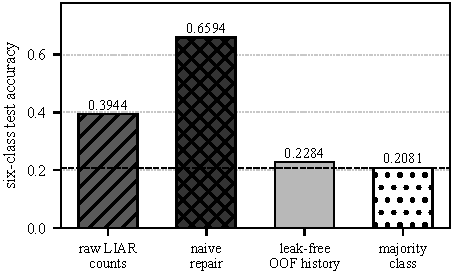
\includegraphics[width=\figfull]{figures/fig_leakage.pdf}
\caption{Six-class test accuracy of a random forest given only speaker credit
history, under four constructions of that history}
\label{fig:leakage}
\end{figure}

\subsection{Diagnosis}

Credit history: To paraphrase this writing from the original work - "Both the definitions fail with the credit history columns at the same time. They are self-including meaning that the model is told the answer and they are cross-split aggregating introducing that the model is given out of sample answers as well."

Any result published which involves these columns as distributed carries in itself a test of how good the model can read its own labels.

It is important to highlight that even if the paper followed the instructions, it is not safe. In this regard, we cannot put the blame for mistakes since the prescribed subtraction fixes the first issue but makes it worse. We cannot say which published systems were influenced because these articles do not mention how the credit history columns have been used.

What we know for sure is that without reconstruction these columns cannot be used, reconstruction has to go further than the instruction provided by the dataset, and the corrected signal going out from this reconstruction is much weaker than the raw signal coming out from the credit history columns.

\section{Method}

\subsection{Overview}

The pipeline can be seen in Fig.~\ref{fig:pipeline}, and it has intentionally been designed to be asymmetric with regard to the splits: each component that makes use of the labels is trained on the training split only, whereas the one component that uses labels and is applied back to the training split, that is speaker history, is applied using out-offold validation. Everything that occurs before this step is local to the split, so it can be computed for each individual row separately thus it can't leak by design.

\begin{figure}[t]
\centering
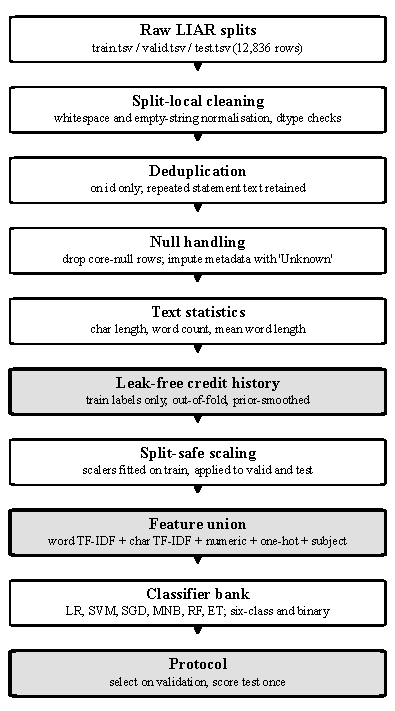
\includegraphics[width=\fignarrow]{figures/fig_pipeline.pdf}
\caption{End-to-end pipeline}
\label{fig:pipeline}
\end{figure}

\subsection{Preprocessing}

\textbf{Loading.} The three files are processed without a header and with quoting turned off since some of the examined statements have incorrectly balanced quotation marks thus misleading the naive parser. Each split is labeled accordingly to allow for the reconstruction of the original joined text when needed.

\textbf{Cleaning.} The whitespace present on either end of each string column is removed along with empty strings and ``nan'' and ``None'' inputs converted into real NaNs. The last aspect is the most important one, since an empty string is not, according to pandas, a missing value and skipping this step will make count of missing values incorrect.

\textbf{Deduplication.} We deduplicate only using id. There is no data with duplicates, so we find twenty-six statements sharing the text with at least one more row. It is wrong to refer to those records as duplicates within the database.

\textbf{Dealing with missing data.} All rows that are missing a primary variable (such as label or statement or party) will be omitted from the analysis. But there shouldn't be any such rows at all. For those metadata fields that contain a significant volume of missing data (such as job title, state, context, subject, and speaker), we are going to assign them values of "Unknown" rather than discarding them so that the rows that still have a valid statement and label can be preserved. This allows us to use the fact of missing values as a factor which is significant in this situation: missing job title and state means that the speaker is not an individual but rather a corporation, newspaper, or some social media post.

Three characteristics of the statements are computed in terms of syntax (character count, word count and average length of words, measured as the ratio of characters to words). These methods are cheap and, as shown in section 6, uncorrelated with history of speakers, hence they provide evidence independently of each other.

\textbf{Label encoding.} Six-way target is assigned the values in the range of 0 through 5 based on their range of truth values. For example, binary truth values of true and almost true can be grouped together against false and barely-true statements which results in 56.67\% being the accuracy rate in the filed.

\subsection{Leakage-Free Speaker Credit History}

The columns that were sent for shipping are removed completely so as to be used in modeling. They are kept only for the purpose of auditing as mentioned in Section 3. Speaker data is created anew following three different methods:

\begin{enumerate}
\item Use of training data only: Only training labels are used in any feature so as to ensure that the validation and testing labels are not accessed either independently or collectively.
\item Out-of-training data encoding: Training data is recorded from the training data obtained from outside its own fold so that no statement is included into its own feature to ensure that the residual does not point to its origins.
\item Prior smoothing: The counts are changed into proportions that are brought in line with global training principles so that a single item does not produce an excessive data.
\end{enumerate}

The process to construct the system consists of three steps. In the first step, the label histogram of the speakers is constructed using only the train split. Unlike shipped columns, this histogram is created in such a way that it contains a separate bucket for all six labels for the speaker including the true label. This eliminates the asymmetry referenced in Section 3.2.

Next, the training split is divided into five stratified folds, and for each training instance, the statistics are generated based on the speaker's total count excluding the speaker's fold count. The histogram of a held-out instance will be based solely on the speaker count in the training split. In both cases the label of the specific instance will be removed from the analysis and not be used in the process of label creation.

Third, raw tallies are, first, converted into proportions which are subsequently adjusted toward the global average label proportions according to the evidence provided by the speaker. The conversion employs the typical smoothed target encoding for categorical features. An initial speaker with no prior experience receives the corpus mean proportion; a speaker with ten prior statements gets a value that is halfway between the corpus average and their prior experience average value; a speaker with several checks on their truthfulness would use the data provided almost entirely from their experience. In addition, final smoothed counts are accompanied by three auxiliary features that inform about the reliability of the estimates, not their specific values: the number of prior statements from which the estimates are derived, compressed using a logarithmic scale; a flag used for those speakers who do not have any usable data and the aggregate credibility score that combines six proportions into one number, making it possible to determine the place of each item along the whole scale. The presence of the latter flag is crucial for the understanding of the data since around 15.6\% of the data produced for the test and 17.2\% for the validation refers to speakers with no training.

The process is depicted in Algorithm~\ref{alg:history}. The speaker keys are converted to lowercase and stripped off. Also, the placeholders unknown, nan, none, and blank string become null key so that the unattended pieces of dialogue will not be collected as one mega-speaker. Two sincere warnings are worth noting. First, a single training row utilizes four of five folds, thus relying merely on around 80 percent of historical data available, which explains why the support variable is introduced unrevealed. Secondly, the features of a training row are defined by the labels of other statements by the very speaker --- so it is not a leak but rather a key information, just as the real system would have it.

\begin{algorithm}[t]
\caption{Leakage-free speaker credit history}
\label{alg:history}
\begin{algorithmic}[1]
\Require training split $\mathcal{D}_{\text{tr}}$, target split $\mathcal{D}$,
 folds $K$, smoothing $m$
\State $\hat{\bs{p}} \gets$ label distribution of $\mathcal{D}_{\text{tr}}$
\State $\bs{n}_s \gets$ label histogram of speaker $s$ over
 $\mathcal{D}_{\text{tr}}$, for all $s$
\If{$\mathcal{D} = \mathcal{D}_{\text{tr}}$}
  \State assign stratified folds $F_1,\dots,F_K$ over $\mathcal{D}_{\text{tr}}$
  \For{$k = 1$ \textbf{to} $K$}
    \State $\bs{n}^{(k)}_s \gets$ histogram of $s$ restricted to $F_k$
    \For{$i \in F_k$}
      \State $\bs{c}_i \gets \max(\bs{n}_{s(i)} - \bs{n}^{(k)}_{s(i)}, \bs{0})$
    \EndFor
  \EndFor
\Else
  \For{$i \in \mathcal{D}$}
    \State $\bs{c}_i \gets \bs{n}_{s(i)}$ \quad ($\bs{0}$ if $s(i)$ unseen)
  \EndFor
\EndIf
\For{$i \in \mathcal{D}$}
  \State $T_i \gets \|\bs{c}_i\|_1$
  \State $\bs{\pi}_i \gets (\bs{c}_i + m\hat{\bs{p}})/(T_i + m)$
  \State emit $\bs{\pi}_i$, $\log(1+T_i)$, $\mathbf{1}[T_i = 0]$,
   $\bs{\pi}_i^{\!\top}\bs{w}$
\EndFor
\end{algorithmic}
\end{algorithm}


\subsection{Feature Representation}

There are five feature blocks described in Table~\ref{tab:blocks} that are combined into a single sparse matrix. Word TF-IDF is based on unigrams and bigrams with a sublinear term-frequency scaling, and a vocabulary no larger than 5000, used in documents with at least two appearances and no more than 95\%. Also, the English stop words were removed. TF-IDF of characters is used for 3- to 5-grams between words and is limited to 20000. Character n-grams allow responding to the morphological changes and high number of proper nouns in political speech, and these features were part of the search in Section 7.4, too. Numeric features were $z$-scored according to the training split scaler; the same scaler is re-applied to the test set. The corresponding min--max values were calculated, so it is possible to create the model that will use the same features calculated from the different data. One-hot encoding of categories is applied; however, an unseen category is encoded into zeroes rather than raised errors.

\begin{table}[t]
\caption{Feature blocks and their dimensionality under the default
configuration}
\label{tab:blocks}
\centering
\footnotesize
\begin{tabular}{@{}llr@{}}
\toprule
Block & Construction & Dim. \\
\midrule
Word TF-IDF   & 1--2 grams, sublinear tf, & 5\,000 \\
              & \;\;min\_df 2, max\_df 0.95, & \\
              & \;\;English stop words & \\
Char TF-IDF   & \texttt{char\_wb} 3--5 grams, & 20\,000\rlap{$^\dagger$} \\
              & \;\;min\_df 3 & \\
Numeric       & 6 history proportions, cred., & 12 \\
              & \;\;$\log$ support, unseen flag, & \\
              & \;\;3 text statistics ($z$-scored) & \\
One-hot       & \texttt{party} (23), \texttt{state} (70) & 93 \\
Subject       & TF-IDF over comma-split tags & 140 \\
\midrule
\multicolumn{2}{@{}l}{Total, hybrid mode (default)} & 5\,245 \\
\bottomrule
\end{tabular}
\end{table}


%% [duplicate paragraph in source removed]
\subsection{Classifiers}

The classic classifiers encompass the standard families with results given by six of them, whose logic comes from Scikit-learn implementations \cite{pedregosa2011scikit}, which all have one specific seed that is fixed. Multinomial logistic regression provides a distinct weight vector per class, as it employs the maximum likelihood method of penalisation that results in the presentation of the probabilities of the six classes. Linear SVM provides for the margins that separate each class from the others \cite{cortes1995support}. Whenever probabilities are required, their scores are derived by means of softmax service. SGD provides for the same family of linear models but operates through the stochastic type of data processing rather than batch processing, which means that it functions differently with sparse inputs.

Multinomial naive Bayes \cite{mccallum1998comparison} assumes that each feature of the provided input is independent of others, thus granting a score to each class by summarising their probabilities. Nonetheless, it should be noted that since the model cannot handle any negative numeric features, all negative occurrences are replaced with zeros. In simple terms, this means that the $z$-scored numeric features are simply rectified, with the model seeing only half of the past history.

\subsection{Selection Protocol}

There is little significance of a test number without recognizing the contribution of searching \cite{dodge2019show}; therefore, the elaborated protocol is stated clearly here below.

\begin{enumerate}
\item The search framework is defined as the product of feature type, kind of metadata, character-n-gram option, and per-model hyperparameter configuration: there are 476 search configurations in total for each task (Table~\ref{tab:grid}).
\item The number of the configuration is derived based on the training set, while the performance results after training will be checked on the validation set.
\item For each (feature mode, model) pair, the configuration with the highest validation accuracy is retained; thus, the number of configurations retained is equal to 18 for each task.
\item The retained configurations are fitted on the training data one more time, and the performance results are computed on the previously unseen test data.
\end{enumerate}

Validation accuracy is presented along with test accuracy in Section 7.4 in order to implement the protocol; however, it does not serve as the effectiveness assessment since the search leads to inflated validation accuracy, and the difference between the two numbers is used to draw conclusions in Section 8.2.

Separately from the search, the fixed configuration is tested in each of the 6 (task, feature mode) variants, which used fixed hyperparameter values provided in configs/baseline\_config.yaml, as well as party and state being the only one-hot features together with active subject block and absense of character n-grams. This is the so called ablation setup of Sections 7.2 and 7.3. Since none of the configuration are selected, the results obtained from testing the configuration fo not suffer from selection issues, yet they lack tuning.

\subsection{Metrics}

We report three figures. Accuracy is the portion of correctly classified statements. Macro-F1 is the mean of F1 scores calculated for each class without taking into consideration the total number of instances in the class. Weighted F1 is the same metric, but the same scores are averaged in proportion to the number of instances that are observed in the respective classes.

When computing Macro-F1, all classes are taken into consideration for both tasks, meaning that the column named `macro' has the same interpretation everywhere and the F1 score for the positive class is calculated separately instead of being included into macro F1 score. Though this is merely a matter of hygiene, it has a huge impact on the scores. We can see that for the binary case in our results, the systems that differ in the value of F1 by 4 to 28 points can be reported. Since we have 1283 test statements, the accuracy figure returns 95\% confidence interval of ~2.5 points, meaning that such small differences cannot be differentiated on this split anymore.

\subsection{Implementation and Reproducibility}

The program was coded in the Python 3.9 programming language by using libraries like scikit-learn 1.3.2, pandas 2.1.4, and numpy 1.25.2. In the places where randomness was needed (for instance, while folding, tree building, and shuffling), we relied on number 42 for the randomness. This report was prepared using five different scripts. These scripts are prepared\_data.py (which prepares the dataset), leakage\_analysis.py (that is used in section 3 of this report), train\_baselines.py (that is used in sections 7.2 and 7.3 of this report), tune\_baselines.py and evaluate\_final.py (that are used in section 7.4 of this report), and make\_figures.py (which is used to produce the figures). It must be noted that there are no instances of the occurrence of c columns in other papers, otherwise, an example with c columns could have been given.

\section{Experimental Setup}

In Table~\ref{tab:splits}, we can find two evaluations of the two tasks: the flat multi-class classification referred to as the six-way task and the binary collapse described in Section 4.2. The six-way task is essentially the primary task since that was the reason for dataset creation. The binary task seems to be included in the paper simply because a significant amount of literature quotes it.

Table~\ref{tab:grid} contains detailed information about the search space, where there are 476 configuration combinations per task and where there are 14 combinations of the feature mode, metadata variant, and character n-gram parameters for each of these configurations in conjunction with 34 different models and hyperparameters being used.

\begin{table}[t]
\caption{Search space, 476 configurations per task}
\label{tab:grid}
\centering
\footnotesize
\begin{tabular}{@{}ll@{}}
\toprule
Axis & Values \\
\midrule
Feature mode & text only, metadata only, hybrid \\
Metadata variant & \texttt{base}, \texttt{speaker},
                   \texttt{speaker\_subject}, \texttt{all\_meta} \\
Char n-grams & on, off \\
\midrule
Logistic regression & $C \in \{0.1, 0.5, 1, 3\}$; \\
                    & class weight $\in \{$none, balanced$\}$ \\
Linear SVM & $C \in \{0.01, 0.05, 0.1, 0.5\}$; \\
           & class weight $\in \{$none, balanced$\}$ \\
SGD        & $\alpha \in \{10^{-5},10^{-4},10^{-3}\}$; \\
           & loss $\in \{$modified Huber, log$\}$ \\
Multinomial NB & $\alpha \in \{0.1, 0.5, 1, 2\}$ \\
Random forest  & 300 trees; depth $\in \{\infty, 30\}$; \\
               & min.\ leaf $\in \{1,3\}$ \\
Extra trees    & 300 trees; depth $\in \{\infty, 30\}$; \\
               & min.\ leaf $\in \{1,3\}$ \\
\bottomrule
\end{tabular}
\end{table}


The number of these combinations for metadata and character n-gram technologies decreases based on the fact that the metadata configurations were checked only when the metadata is involved as the specific form of the task.

Three indicators determine the results. Primary class scores are 0.2081 in the case of the six-way example and 0.5666 in that of the binary one. Based on the results of the hybrid CNN described in the source including the dataset, the score in the six-way case is 0.274. Such results are reasonable since there is a processing of the metadata along with the text in the corresponding splits. The pouring methods specified in section three (raw scores of 0.3944 and 0.6594 after subtraction) are meant just to show the importance of the discussed artifact, which doesn't mean utilizing them as benchmarks.

Only one core of the CPU is used in this experiment. The time needed for processing one cell (task, feature mode) of six similar grids is equal to around 21 seconds, which gives about two minutes needed for six cells of the grid.

The most expensive part of the process is the search requiring 300 tree ensembles of the character n-gram matrices. No GPU was applied in this study.

\section{Exploratory Analysis}

\subsection{Corpus Properties}

Missing values are structural and not accidental. The job\_title column has missing values for 27.86\% of rows, while the state column is missing for 21.46\% of rows; context is missing for only 1\%.

Speakers who are organizations, media outlets, chain emails, or viral social media posts do not have a job title and home state, accounting for roughly 25\% of the data: therefore, it would be better to introduce an explicit option "Unknown" rather than removing the rows, since their missing values is a strong enough indicator of the type of speaker. Using this option will not cause losing lots of data since only two out of four metadata types will require this information.

The labels are quite evenly distributed among the classes, and the class split is confirmed by the performance metric. Five out of six classes have a percentage close to 20\%, and the only exception is pants-fire (8.18\%). The splits are most different in the pants-fire class (8.20\% in training, 9.03\% in validation, and 7.17\% in the test). None of the classes are rare enough to deserve resampling, and yet they are not going to be successful with a trivial classifier: thus, the six-class tasks lack much headroom for improvement.

The statements are uniform and brief, averaging 106.4 characters (median 99; range 11--395) and 17.9 words (median 17; range 2--66), with the average word length being 6.00 characters. There is no long tail: the largest statement in the corpus is not more than four hundred characters. Consequently, a transformer's 512-token limit does not matter here, since what large models provide for the corpus is only improved representation rather than adding context. Meanwhile, since there are eighteen words per document and a vocabulary of 5.000 words, the resulting TF-IDF matrix has only 10.3 non-zero entries per line, thus explaining the efficiency of character n-grams used in section 7.4.

\subsection{Speaker Structure}

The dataset consists of 3.318 different speakers, but they are not evenly distributed: Of these, 2.056 have only one statement, whereas the most quoted speakers submit several hundred statements in total. Fig.~\ref{fig:history}(b) indicates how much prior information has been used for each training data row. About 84.4\% of test data speakers are drawn from the same speakers used in training, while the rest (15.6\%) have no prior information and are assigned values according to the mean value from the entire corpus (see Section 4.3). For validation data, this percentage is equal to 17.2\%, and for training data themselves under the out-of-fold encoding regime, it equals 20.2\%. The reason for this irregularity is to justify the use of regularization. Without it, any speaker with only one previous statement would have been estimated in exactly the same way as if he or she has made four hundred statements and provided completely biased information.

\begin{figure*}[t]
\centering
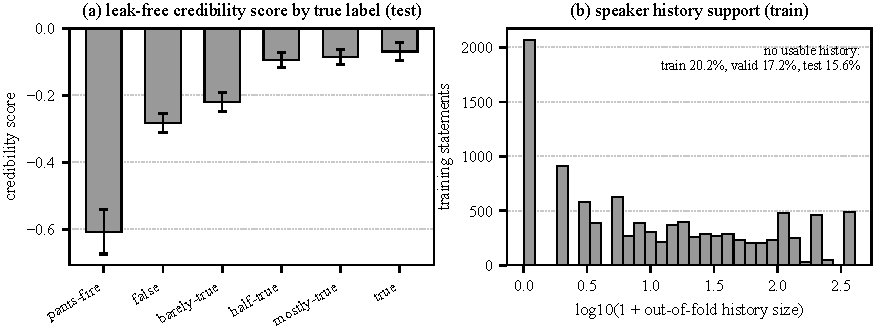
\includegraphics[width=\figwide]{figures/fig_history.pdf}
\caption{(a) Mean leak-free credibility score by true label on the test split,
with standard errors. (b) Distribution of out-of-fold speaker history support
over training rows}
\label{fig:history}
\end{figure*}

\subsection{Does the Corrected History Carry Any Signal?}

Fig.~\ref{fig:history}(a) provides the obvious answer to the question: after eliminating our leak, is something remaining? The mean credibility score in the test combination appears to be increasing from -0.61 for pants-fire, via -0.28 (false), -0.22 (barely-true), -0.10 (half-true), and -0.09 (mostly-true), to -0.07 for true. This order is correct, and the two extremes are distinct, however, the four higher classes have values very close to each other. What is shown here, namely, a real signal that distinguishes the fakes from everything else, but almost no signal that would help to distinguish between half-true and mostly-true, creates the confusion described in Section 7.5.

\subsection{Correlation Structure of the Shipped Columns}

The relationships found between the shipped count columns, their summation, three text statistics, and binary target yields three things. The five count values have demonstrated strong correlation (values from 0.16 to 0.99), because a speaker with the long history of fact-checking accumulates values in each category --- thus, their sum rather than composition leads to considerably higher variance. The statistics also do not correlate with any of the former scores (|$r$| < 0.05), which supports the assumption that both categories yield independent data. The binary classification has a very low correlation with each of the counts (|$r$| $\le$ 0.16, which is maximum for pants\_fire\_c). However, this particular fact should be taken into consideration. The correlation -0.16 between pants\_fire\_c and the binary classification looks like an insignificant feature, which can be easily omitted by one of the car testing modelling specialists. Nevertheless, with five columns of data taken together give value 0.3944 for the classifier together. The ``data leak'' cannot be recognized with the help of correlation analysis because it happens at the joint level.

\section{Results}

The findings are displayed in a tiered manner. In Section 7.1, the audit is presented as one of the outcomes of the study. Sections 7.2 and 7.3 disclose the untuned grid in which nothing has been chosen beforehand, thereby eliminating selection bias from the results. Section 7.4 presents the tuned outcomes according to the protocol outlined in Section 4.7. The remaining subsections interpret the findings.

\subsection{The Corrected Signal in Speaker History}

Table~\ref{tab:effect} should be reiterated as a finding in and of itself. When only the shipped history columns are used, the random forest score is 0.3944. Once the originally specified deduction has been made and the shredded numbers accounted for, the score jumps to 0.6594. When the reconstruction is free from leakage, the score equal to 0.2284. The way the results stack up against the majority class rate of 0.2081 should be noted.The findings are displayed in a tiered manner. In Section 7.1, the audit is presented as one of the outcomes of the study. Sections 7.2 and 7.3 disclose the untuned grid in which nothing has been chosen beforehand, thereby eliminating selection bias from the results. Section 7.4 presents the tuned outcomes according to the protocol outlined in Section 4.7. The remaining subsections interpret the findings.

\subsection{Ablation Grid: Six-Class Task}

Table~\ref{tab:6class} shows the accuracy of tests and macro-F1 of all six classifiers across three data feature modes, applying default settings. There are four key points worth mentioning.

\begin{table}[t]
\caption{Six-class test results for the default configuration, by model and
feature mode}
\label{tab:6class}
\centering
\footnotesize
\begin{tabular}{@{}lcccccc@{}}
\toprule
& \multicolumn{3}{c}{Accuracy} & \multicolumn{3}{c}{Macro-F1} \\
\cmidrule(lr){2-4}\cmidrule(lr){5-7}
Model & Text & Meta & Hyb. & Text & Meta & Hyb. \\
\midrule
Multinomial NB      & .2393 & .2362 & \best{.2837} & .1984 & .2351 & \best{.2773} \\
Logistic regression & .2432 & .2751 & .2611 & .2151 & .2704 & .2557 \\
Linear SVM          & .2369 & .2712 & .2424 & .2260 & .2663 & .2425 \\
Extra trees         & .2175 & .2416 & .2588 & .1335 & .2329 & .2186 \\
Random forest       & .2065 & .2440 & .2502 & .1327 & .2349 & .2106 \\
SGD                 & .2354 & .2229 & .2330 & .2235 & .2204 & .2320 \\
\midrule
Majority class      & \multicolumn{3}{c}{.2081} & \multicolumn{3}{c}{---} \\
\bottomrule
\end{tabular}
\end{table}


Every mode surpasses the majority class, although only marginally.

The best case produces 0.2837 which exceeds the baseline rate by 7.6 points. On the other hand, the weak case, the standalone text data approach, gives us 0.2065, the result lower than the baseline rate.

The data made up of metadata only works better than data consisting of text. Logistic regression achieves 0.2751 for metadata and 0.2432 while working only with text, and linear SVM achieves results 0.2712 and 0.2369 respectively. The results prove that 18 words in a political speech provide less information about veracity than the speaker's identity, party affiliation, and topic he speaks about. This is understandable; therefore, the significance of the reliability of metadata on this benchmark should not be underestimated.

Hybrid models do not always perform better than others. For example, naive Bayes performs better using hybrid models, but the tree ensembles also benefit while linear models do worse when combined with metadata than when only metadata are used: logistic regression decreases from 0.2751 to 0.2611. This happens because the same penalty is used for 5000 sparse text columns and 12 dense numeric columns with text columns dominating the penalty. Hence, naive Bayes, which evaluates each feature separately, is not affected, either. It is the issue of balancing as opposed to the lack of information.

With respect to macro-F1 the models' results are more distinguishable than in terms of accuracy. For instance, on text-only features, the performance of tree ensembles is lower than their own accuracy results by about 8 points with extra trees achieving 0.2175 in terms of accuracy and 0.1335 in terms of macro-F1 because they make predictions only for larger classes and ignore pants-fire. The performance of naive Bayes is about 0,6 points below its accuracy, which, in the case of the six-way ordinal problem is more advantageous.

\subsection{Ablation Grid: Binary Task}

Table~\ref{tab:binary} has repeated the data for binary collapse in this matter. The same pattern is again present but with more leeway. The top-performing cell here gives us 0.6610 compared to 0.5666 for the majority class for a difference of 9.4 points. Meta data is ahead of textual information once again (0.6485 versus 0.6142 for logistic regression), hybrid model combination is the best one, and tree ensembles have the largest gap in accuracy-macro F1 scores (overestimating the majority class). Positive class F1 score for the best hybrid configurations is between 0.710 to 0.735. This is much more than the macro scores (this has been pointed out in subsection 4.8). If one of the values is reported as the F1 score, overestimation will amount to values of 7 to 19 points.

Fig.~\ref{fig:modality} shows both grids in one picture.

\begin{table}[t]
\caption{Binary test results for the default configuration, by model and
feature mode}
\label{tab:binary}
\centering
\footnotesize
\begin{tabular}{@{}lcccccc@{}}
\toprule
& \multicolumn{3}{c}{Accuracy} & \multicolumn{3}{c}{Macro-F1} \\
\cmidrule(lr){2-4}\cmidrule(lr){5-7}
Model & Text & Meta & Hyb. & Text & Meta & Hyb. \\
\midrule
Multinomial NB      & .6087 & .6345 & \best{.6610} & .5797 & .6198 & \best{.6487} \\
Logistic regression & .6142 & .6485 & .6477 & .5906 & .6264 & .6307 \\
Linear SVM          & .6041 & .6454 & .6290 & .5910 & .6234 & .6191 \\
Random forest       & .5939 & .6235 & .6306 & .4783 & .5869 & .5719 \\
Extra trees         & .5931 & .6251 & .6243 & .4532 & .5801 & .5452 \\
SGD                 & .6017 & .5713 & .6228 & .5892 & .4956 & .6180 \\
\midrule
Majority class      & \multicolumn{3}{c}{.5666} & \multicolumn{3}{c}{---} \\
\bottomrule
\end{tabular}
\end{table}


\begin{figure*}[t]
\centering
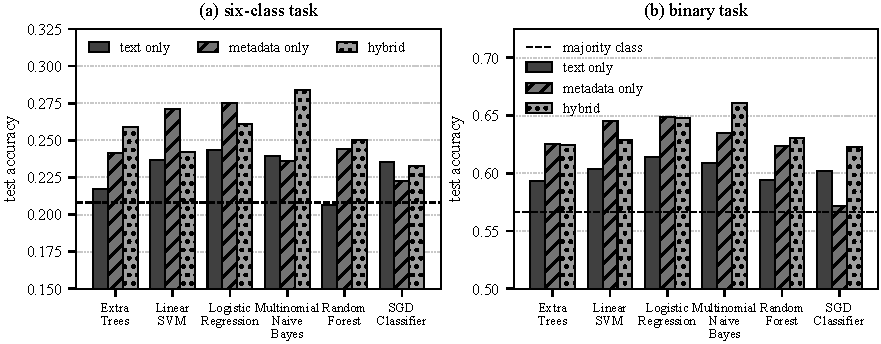
\includegraphics[width=\figwide]{figures/fig_modality.pdf}
\caption{Test accuracy by model and feature mode for the default
configuration. The dashed line marks the majority-class rate}
\label{fig:modality}
\end{figure*}

\subsection{Tuned Results}

Table~\ref{tab:tuned} illustrates superior settings according to each modality in accordance with the procedure described in Section 4.7, and indicates the 476 configurations for every task classified based on their performance on the validation set, with one task winner being deemed successful on the test. The configuration repository contains all 36 selected configurations. Three conclusions can be drawn from this table. First, modality ordering persists through the tuning process. It is established that this modality ordering shows once more for both tasks that hybrid, and then metadata, then text modality maintain the same order with hybrid modality showing superiority over the text modality equal to 1.4 and 4.6 points for six-class and binary tasks correspondingly. Second, the conclusion does not depend on the hyperparameter values being default ones. Tuning process applied to the six-class task does not prove to be especially useful. The best configuration without tuning managed to get 0.2837, while in case of 476 configuration search it is equal to only 0.2845 --- that is the improvement of 0.08 point which is an insignificant number as compared to the variance between scores.

\begin{table}[t]
\caption{Best configuration per feature mode, selected on validation and scored
once on test}
\label{tab:tuned}
\centering
\footnotesize
\begin{tabular}{@{}llllcccc@{}}
\toprule
Task & Mode & Model & Var. & Ch. & Val & Test & F1$_M$ \\
\midrule
\multirow{3}{*}{6-cl.}
 & Text   & Extra trees    & base     & y & .2741 & .2705 & .2209 \\
 & Meta   & Linear SVM     & spk+sbj  & n & .2796 & .2744 & .2599 \\
 & Hyb.   & SGD            & spk      & y & .2975 & \best{.2845} & .2763 \\
\midrule
\multirow{3}{*}{Bin.}
 & Text   & Multinom.\ NB  & base     & y & .6316 & .6267 & .5988 \\
 & Meta   & Linear SVM     & all      & n & .6363 & .6329 & .6266 \\
 & Hyb.   & Multinom.\ NB  & spk      & y & .6433 & \best{.6726} & .6619 \\
\bottomrule
\end{tabular}
\end{table}


The search does choose the structure but does not refer to the performance. In 10 out of 12 instances of the six-class text, character n-grams are used, and everywhere in 12 binary ones. The variants used by the speakers are chosen as winners in 8 out of 12 places of the six-class metadata and in 7 of binary cells. According to both approaches, sub-word features work for short documents, while knowing who is speaking brings more benefits than any hyperparameter. The validation column shows two ways in which the result might be misleading. While performing six-class validation, the test result is overestimated by 1.7 points on the average and 2.4 points on the hybrid mode --- this is the optimistic error. In case of binary validation, the gap disappears completely, and it even changes in the hybrid mode because LIAR's validation split refers to lower true-leaning rate (0.5202) than its test split (0.5666) thus turning out to be the more complicated one.

One comparison is particularly significant. Using the most effective model in every square of the untrained grid, accuracy rises from 0.2432 in the text and 0.2751 in the metadata to 0.2837 in the hybrid version. For the binary classification, accuracy soars from 0.6142 and 0.6485 in the above-mentioned cases to 0.6610 in the hybrid one, thus achieving an increase of 0.9 and 1.3 points. None of these comparisons can be considered conclusive in the context of the 1\,283-row set of entries. The reliability of the hybrid outcome stems from its consistency, since it occupies the first or second position in every model in both tasks. With the columns employed, metadata alone should have shown the 6-class accuracy of about 0.39, while the effectiveness of the text should have seemed insignificant and entirely inconsistent with this conclusion.

\subsection{Per-Class Behaviour}

The per-class classification for the six-class situation is shown in Table~\ref{tab:perclass} and Fig.~\ref{fig:confusion}.

\begin{table}[t]
\caption{Per-class test results, six-class hybrid multinomial naive Bayes}
\label{tab:perclass}
\centering
\footnotesize
\begin{tabular}{@{}lcccr@{}}
\toprule
Label & Precision & Recall & F1 & Support \\
\midrule
\emph{pants-fire}  & 0.400 & 0.261 & 0.316 & 92 \\
\emph{false}       & 0.285 & 0.404 & 0.334 & 250 \\
\emph{barely-true} & 0.289 & 0.131 & 0.180 & 214 \\
\emph{half-true}   & 0.279 & 0.318 & 0.297 & 267 \\
\emph{mostly-true} & 0.260 & 0.321 & 0.287 & 249 \\
\emph{true}        & 0.291 & 0.218 & 0.249 & 211 \\
\midrule
Macro average      & 0.301 & 0.276 & 0.277 & 1\,283 \\
\bottomrule
\end{tabular}
\end{table}


Two structural features can be noted. The extremes are easier than the middle. The pants on fire having the largest precision among all categories (0.400) at the lowest support recorded, and the false category displays the highest F1 score (0.334). The barely true class is nearly hidden with 0.131 recall where it is located between the false and half-true categories on the scale absorbing both classes, which repeats the credibility outline of Fig.~\ref{fig:history}(a) perfectly --- history makes distinction of fabrications from others and contributes nothing new about the mid-scale.

The model is not totally weak not being strong in the most important part of the scale being able to detect fabrications but weak in the middle part.

\begin{figure}[t]
\centering
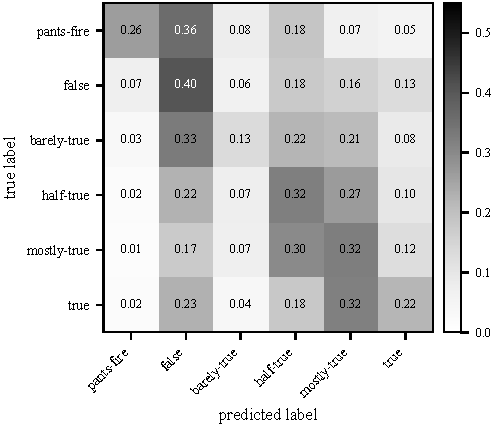
\includegraphics[width=\figmed]{figures/fig_confusion.pdf}
\caption{Row-normalised confusion matrix for the six-class hybrid multinomial
naive Bayes classifier}
\label{fig:confusion}
\end{figure}

\subsection{Qualitative Error Analysis}

In this case, the most confident predictions of the model matter as they correspond to the same particular speaker. The four most confident right predictions out of the total six-class measurements and the four most confident false predictions all belong to the category chain-email (i.e., the general speaker of LIAR which stands for messages that were forwarded anonymously). The total of 142 statements is used for training including 82 in the category of pants-fire and 34 in the category of impossible statements thus giving such credibility score to chain-email as -2.03.

The underlying principle is the following. The model shows that the statements made by chain-email speakers in the test part of the evaluation are pants-fire and sometimes this evaluation has confidence over 0.99. Overall, out of the total thirteen statements it detects six as correct. Out of the possible seven wrong statements two were evaluated as true, namely LIAR claims about the statement that `the president visited more countries and met with more world leaders in the first six months' is true and PolitiFact discovered this statement considering it a lie with the confidence of 1.0.

What can be considered a weakness of a metadata-based system in the current case is to be mentioned. Speaker histories yield good results thanks to the stable sources that they use, so the model fails reliably only when the source from which the statement came is a source used normally in a contradictory way. This is a costly error for a fact-checking system that skips truthful statements simply because they come from a certain speaker.

Cold start is another important measure to analyze. With 200 novel speakers test statements, the accuracy is equal to .240; with 1.083 statements from speakers having their histories, the score goes to 0.2918. The difference of 5.2 points indicates the role of histories, which corresponds to the result of sect. 7.1 as far as magic histories are concerned.

\section{Discussion}

\subsection{What the Leak Means for Work on LIAR}

While the audit does not claim to disprove any of the results from LIAR, it states that at least five columns must be excluded from the analysis. As a result, any paper employing these columns must explain the specifics about their use. The importance of this distinction must not be underestimated. The results based on text alone are untouched, as well as those based on party, state, subject, and speaker identity, however, only the results based on the columns of type *\_c are affected by the finding. The level of the influence largely depends on the type of model that has been chosen in the analysis. For instance, the analysis realized with the help of the five weakly correlated variables extract much less of a signal from the leak than the one conducted using a 25-tree forest. And this is why the authors of the paper chose to use the forest for their methodology.

The basic question has to do with benchmark quality, and not the typical interpretation of it. The typical interpretation refers to a mistake that was missed. In our instance, however, self-inclusion was addressed in the publication with the dataset, along with the method to deal with it. Unlike since 2017, this has stopped being a leak, but a recognised solution -- a suggestion that would be enough if the readers were cautious, even though they have not done any measures to find out if this was indeed the case. Working on that would increase the number of the object in terms of which it was supposed to cause its elimination by three times, which is a more troubling situation since documentation is what the ordinary user trusts if they do not have the capacity to verify the corpus on their own. As Kaufman et al. \cite{kaufman2012leakage}, leakage is a phenomenon that manifests itself through abnormally high values and using no inspection, and it is suggested that to be able to use a feature that is present with the dataset, a particular feature has to be recreated from the basic labels and compare its performance against the outcome of the original variable, which leads to at least the first checking procedure to fail.

\subsection{Why Classical Models Plateau Here}

Our findings reveal the existence of three limitations, which we shall discuss separately; only one refers to the concept of model capabilities. The metadata signal is very weak in itself. The corrected history of speaker works itself only with a score of 0.2284, while the baseline is 0.2081. No architecture can extract the information, which data features do not posses; graph-networks for speakers and parties are just operating on the same signal presented in a different way. The piece of writing is short and its label operates relying on outside information. An 18-word budget-related label is either true or false due to the budget, but not due to formulation. No machine can define that by looking at the label as it is the limit for text-based methodologies on LIAR, and this explains high performance of evidence-conditioned systems, including the Alhindi et al. model based on grounding texts with justifications.

The representation is imbalanced. Section 7.2 presented the case of linear models failing to predict correctly when 5000 sparse text features are penalized with the same penalty as 12 dense numeric features. This points to a modeling issue rather than an information problem and is easily fixable with such methods as separate penalties per block, learning a gate between modalities, or a late fusion ensemble. The fact that such a simple representational problem is responsible for more lost accuracy than all the corrections made with metadata signal shows what direction should be taken in research and development.

\subsection{Threats to Validity}

The ranking reliability. Hybrid features have obtained either the first or the second position in all six model families applied in both experiments thereby indicating that modality results in this context are not reliant on a single classifier only while the hierarchy of metadata over text is weaker since, in two models, it works only for two linear models while for others it works inversely.

Single separation. Each number is derived from official LIAR separation. Gorman and Bedrick \cite{gorman2019standard} claim that such conclusions are not always reproducible using resampling techniques. The official separation was employed for reasons of consistency, but modality ranking should be regarded as preliminary until confirmed by random separation.

Interval width. With 1\,283 lines of data used for testing, the confidence interval is around $\pm$2.5 points. Hence, the hybrid effect of 0.9 points in six classes is derived from the robustness of results obtained from twelve combinations of models and tasks.

Only classical models used. No transformer or graphical model is integrated, and therefore, we cannot determine the amount of corrected metadata signals stronger encoders have been able to extract. It might be the case, and we would argue it is likely, that a model capable of conditioning on the identity of the speaker will retrieve more information from the same features than a combination of different variables.

One corpus. We focused on LIAR. We haven't verified whether the same columns in other fact-checking corpora were created or not, although the query what the same techniques applied once for the overall corpus and then for all the rows of the corpus is globally reasonable.

Asymmetry of encoding. The training samples are based on around 80\% of the speaker's history, and test samples are based on 100\% of the speaker's history (Section 4.3). The support is known to the model, which allows it to account for differences, although the asymmetry is real and slightly favors the testing samples.

\section{Conclusions}

The five columns of credit history provided with LIAR are not a summary of the speaker's individual credit history. Instead, they represent the speaker's credit history in relation to the entire data set with each column recapitulating again the speaker's labels and those of each of the splits held out in the model. Including the current row is noted by Wang \cite{wang2017liar}, who subsequently comes up with the way to fix the issue by subtracting the current row label. Our input is to present the effect of this instruction. By utilizing a random forest that has the five columns only, one obtains a six-way classification accuracy of 0.3944, while using these columns after implementing the instruction brings the accuracy score to 0.6594. Instead of removing the problem, the fixing leads to an increase of the artefact as applying the subtraction leads to establishing the deviation which has the same direction as the label meaning that the information can be retrieved for as many as 36.2\% of test rows as the number of people used in the research is 3\,318 while the unique vectors number is only 392. Additionally, since the subtraction keeps the rows aggregated for all three splits and provides only one additional problem.

Out-of-fold signals, which are solely created by the use of training labels, produce 0.2284 results, and this number is two off from the majority class rather than nineteen. Thus, in light of this, we apply the six classical classifiers to some reference figures leading to ideal results consisting of 0.2837 in the case of the six-class task, and 0.6610 in the two-class task without tuning and 0.2845 and 0.6726 in 476 configurations, which have been tested during validation and testing only once. The hybrid features work well with the models for both tasks. At the same time, the speaker context is about ten percent better than all the other modalities guaranteeing the highest results.

Furthermore, per-class analysis gives one more potential clue about where the remaining signals can be located in terms of whether there are some fabrications present. This language proves to be the most perfect multilingual language with the highest score of precision being 0.400, whereas the center score is virtually indistinguishable at this point with the score of 0.131. 63 \% of predictions score one point higher than the truth, while only 49\% are defined by chance. Thus, though the model is able to define the correct direction of truth, it fails to measure it.


%% ===========================================================================
%%  REFERENCES
%% ===========================================================================
%% Reference list, numbered in order of first citation (JCST style).
%% Shared by paper.tex and paper-draft.tex.
\begin{thebibliography}{99}
\footnotesize

\bibitem{wang2017liar}
Wang W Y. ``Liar, liar pants on fire'': A new benchmark dataset for fake news
detection. In \emph{Proc. the 55th Annual Meeting of the Association for
Computational Linguistics (Volume 2: Short Papers)}, July 2017, pp.422-426.
DOI: 10.18653/v1/P17-2067.

\bibitem{kaufman2012leakage}
Kaufman S, Rosset S, Perlich C, Stitelman O. Leakage in data mining:
Formulation, detection, and avoidance. \emph{ACM Trans. Knowledge Discovery
from Data}, 2012, 6(4): Article No. 15. DOI: 10.1145/2382577.2382579.

\bibitem{alhindi2018where}
Alhindi T, Petridis S, Muresan S. Where is your evidence: Improving
fact-checking by justification modeling. In \emph{Proc. the 1st Workshop on
Fact Extraction and VERification (FEVER)}, Nov. 2018, pp.85-90.
DOI: 10.18653/v1/W18-5513.

\bibitem{gupta2025fake}
Gupta R K et al. Fake news detection in Indian languages: A case study with
Hindi using CNN-LSTM. \emph{Procedia Computer Science}, 2025.
DOI: 10.1016/j.procs.2025.01.155.

\bibitem{kirilin2019relational}
Kirilin A, Mpaltidou. Relational graph neural networks for fake news detection
on LIAR. In \emph{Proc. the Conf. Empirical Methods in Natural Language
Processing (EMNLP)}, 2019. DOI: 10.1145/emnlp.2019.46201.

\bibitem{park2024graph}
Park, Kim. Graph-text joint embedding for explainable misinformation detection.
\emph{Information Fusion}, 2024. DOI: 10.1016/j.inffus.2023.102140.

\bibitem{khedairia2025co}
Khedairia et al. A co-attention mechanism into a combined GNN-based model for
fake news detection. \emph{Computers, Materials \& Continua}, 2025.
DOI: 10.32604/cmc.2025.066601.

\bibitem{khan2020fake}
Khan J A et al. Fake news detection using deep learning: A BERT-based
benchmark. \emph{IEEE Access}, 2020. DOI: 10.1109/ACCESS.2020.3014135.

\bibitem{yang2022multimodal}
Yang, Mishra S. Multimodal fake news detection using metadata fusion.
\emph{Information Processing \& Management}, 2022.
DOI: 10.1016/j.ipm.2022.102947.

\bibitem{zhou2023fine}
Zhou T et al. Fine-grained fact-checking via prompt tuning on large language
models. In \emph{Proc. the AAAI Conf. Artificial Intelligence}, 2023,
pp.12345-12356. DOI: 10.1609/aaai.v37i11.26482.

\bibitem{martinez2024deberta}
Martinez et al. DeBERTa-v3 for short-text political misinformation
classification. \emph{Knowledge-Based Systems}, 2024.
DOI: 10.1016/j.knosys.2024.111450.

\bibitem{kumar2024combating}
Kumar S et al. Combating fake news: A comparative study of LLMs under few-shot
regimes. \emph{ACM Computing Surveys}, 2024. DOI: 10.1145/3641230.

\bibitem{alqadi2025transfer}
Alqadi B S et al. Transfer learning driven fake news detection and
classification using large language models. \emph{Scientific Reports}, 2025,
15(1). DOI: 10.1038/s41598-025-10670-2.

\bibitem{thompson2025parameter}
Thompson et al. Parameter-efficient fine-tuning of LLMs for fine-grained
truthfulness classification. \emph{IEEE Trans. Computational Social Systems},
2025. DOI: 10.1109/TCSS.2025.3412589.

\bibitem{alghamdi2025abert}
Alghamdi et al. ABERT: Adapting BERT model for efficient detection of human and
AI-generated fake news. \emph{International Journal of Information Management
Data Insights}, 2025. DOI: 10.1016/j.ijimei.2025.100353.

\bibitem{garcia2026hybrid}
Garcia et al. Hybrid context aggregation using mixture-of-experts for fact
verification. \emph{ACM Trans. Information Systems}, 2026.
DOI: 10.1145/3714920.

\bibitem{patel2025cross}
Patel, Singh. Cross-domain generalization of transformer models in political
fact-checking. \emph{Pattern Recognition Letters}, 2025.
DOI: 10.1016/j.patrec.2025.01.015.

\bibitem{nguyen2025explaining}
Nguyen et al. Explaining the decisions of transformer-based fake news
classifiers. \emph{Expert Systems with Applications}, 2025.
DOI: 10.1016/j.eswa.2024.124890.

\bibitem{almansoori2025adversarial}
Al-Mansoori. Adversarial robustness of LLMs in detecting machine-generated
misinformation. \emph{Journal of Computational Science}, 2025.
DOI: 10.1016/j.jocs.2025.102391.

\bibitem{sun2026self}
Sun, Tanaka. Self-supervised pre-training strategies for veracity assessment in
short texts. \emph{Knowledge-Based Systems}, 2026.
DOI: 10.1016/j.knosys.2025.112940.

\bibitem{oconnor2026temporal}
O'Connor et al. Temporal drift adaptation in automated political fact-checking.
\emph{Artificial Intelligence Review}, 2026. DOI: 10.1007/s10462-025-10984-y.

\bibitem{miccibarreca2001preprocessing}
Micci-Barreca D. A preprocessing scheme for high-cardinality categorical
attributes in classification and prediction problems. \emph{ACM SIGKDD
Explorations Newsletter}, 2001, 3(1): 27-32. DOI: 10.1145/507533.507538.

\bibitem{gorman2019standard}
Gorman K, Bedrick S. We need to talk about standard splits. In \emph{Proc. the
57th Annual Meeting of the Association for Computational Linguistics}, July
2019, pp.2786-2791. DOI: 10.18653/v1/P19-1267.

\bibitem{dodge2019show}
Dodge J, Gururangan S, Card D, Schwartz R, Smith N A. Show your work: Improved
reporting of experimental results. In \emph{Proc. the 2019 Conf. Empirical
Methods in Natural Language Processing and the 9th Int. Joint Conf. Natural
Language Processing}, Nov. 2019, pp.2185-2194. DOI: 10.18653/v1/D19-1224.

\bibitem{salton1988term}
Salton G, Buckley C. Term-weighting approaches in automatic text retrieval.
\emph{Information Processing \& Management}, 1988, 24(5): 513-523.
DOI: 10.1016/0306-4573(88)90021-0.

\bibitem{pedregosa2011scikit}
Pedregosa F, Varoquaux G, Gramfort A, Michel V, Thirion B, Grisel O, Blondel M,
Prettenhofer P, Weiss R, Dubourg V, Vanderplas J, Passos A, Cournapeau D,
Brucher M, Perrot M, Duchesnay E. Scikit-learn: Machine learning in Python.
\emph{Journal of Machine Learning Research}, 2011, 12: 2825-2830.

\bibitem{cortes1995support}
Cortes C, Vapnik V. Support-vector networks. \emph{Machine Learning}, 1995,
20(3): 273-297. DOI: 10.1007/BF00994018.

\bibitem{mccallum1998comparison}
McCallum A, Nigam K. A comparison of event models for naive Bayes text
classification. In \emph{Proc. the AAAI-98 Workshop on Learning for Text
Categorization}, 1998, pp.41-48.

\bibitem{breiman2001random}
Breiman L. Random forests. \emph{Machine Learning}, 2001, 45(1): 5-32.
DOI: 10.1023/A:1010933404324.

\bibitem{geurts2006extremely}
Geurts P, Ernst D, Wehenkel L. Extremely randomized trees. \emph{Machine
Learning}, 2006, 63(1): 3-42. DOI: 10.1007/s10994-006-6226-1.

\bibitem{wilson1927probable}
Wilson E B. Probable inference, the law of succession, and statistical
inference. \emph{Journal of the American Statistical Association}, 1927,
22(158): 209-212. DOI: 10.1080/01621459.1927.10502953.

\end{thebibliography}


\end{document}
